%\chapter{Arquitecturas}\label{cha:arquitectura}
\chapter{Myro y DuinoBot: Las bases de la propuesta}\label{cha:myro_y_duinobot}

%FIX ME: yo pondría como titulo: Myro y DuinoBot: LAS BASES DE LA PROPUESTAS

%El capítulo 2 describe la arquitectura de DuinoBot, Myro, Remotebot y
%XRemoteBot detallando las mejoras provistas por XRemoteBot.

% FIXME: QUIZAS ESTE CAPITULO PODRÍA IR ANTES DEL ANTERIOR... YA QUE SEGURAMENTE VAS A NOMBRAR Y DESCRIBIR VARIAS COSAS QUE LUEGO NOMBRAS ALLÁ... FIJATE

XRemoteBot tiene una arquitectura compleja que
depende de otras bibliotecas y de software instalado en los robots.
El objetivo de este capítulo es describir la interacción entre los
distintos dispositivos y aplicaciones utilizadas, demarcando el límite
entre el desarrollo realizado para esta tesina con el software ya
existente con el que interactúa.

\section{Myro}\label{sec:myro}

Como se mencionó al comienzo de este informe,
Myro\footnote{\url{http://myro.roboteducation.org/}}
es la biblioteca utilizada para controlar a los robots
``Scribbler''
desde un script Python. Esta biblioteca fue desarrollada por
Institute for Personal Robots in Education (IPRE)
para su uso en cursos de computación introductorios~\citep{kumar_2009}
%%\footnote{\url{http://www.roboteducation.org}}
en distintos niveles
educativos\footnote{\url{http://www.roboteducation.org/schools.html}}.
Si bien el proyecto original fue desarrollado por Microsoft Research,
el software generado es software libre y portable tanto en sistemas Windows
como GNU/Linux.

Myro puede interactuar con los robots de dos
formas diferentes: a través de un cable serial (RS323) o bien usando Bluetooth
con RFCOMM\footnote{\url{https://developer.bluetooth.org/TechnologyOverview/Pages/RFCOMM.aspx}}.
El funcionamiento de Myro requiere que el robot tenga
cargado un firmware determinado que espera las instrucciones desde el puerto
serial con el que cuenta el robot, y una placa llamada IPRE Fluke que se conecta
al puerto serial del robot y cuenta con un adaptador Bluetooth que permite
enviarle comandos de forma inalámbrica a través de este protocolo.

\begin{figure}
    \centering
    \includegraphics[width=.7\textwidth]{figures/diagrama_myro}
    \caption{Diagrama de bloques de Myro}\label{fig:diagrama_myro}
\end{figure}

La figura~\ref{fig:diagrama_myro} muestra la interacción entre los componentes
más importantes de software y hardware desde el script del usuario hasta el
robot.

Cabe destacar que el código de Myro funciona con Python 2.7 pero no con
Python 3. Posiblemente esto se relacione con la decisión del \ipre{}
de desarrollar una nueva biblioteca para controlar a los robots que funcione
en distintos lenguajes de
programación\footnote{\url{http://calicoproject.org/}}. De todas formas se
decidió seguir con Myro por la experiencia del autor de esta tesina
con esta biblioteca.

% FIXME Maybe más adelante
Lamentablemente el servidor SVN oficial donde se publicaban las
actualizaciones de Myro a la fecha de escribir este documento
no se encuentra en funcionamiento, por lo que se utilizó una
copia de este repositorio en
GitHub\footnote{\url{https://github.com/yingted/Myro}} de la cuál
se creó un fork y la reorganizó de forma tal que fuera posible instalar
esta biblioteca desde un entorno Python con un solo comando.
Además se hizo
una pequeña corrección para que el uso del paquete
IDLE\footnote{\url{https://docs.python.org/2/library/idle.html}}
sea opcional ya esa biblioteca sirve para crear interfaces gráficas
y eso no es necesario para este proyecto.

Esta biblioteca (técnicamente un paquete Python) consta de múltiples
módulos y requiere de otros para contar con funcionalidades opcionales
como el soporte de joysticks, una interfaz gráfica para mostrar
los valores de los sensores en un diálogo y soporte para manipulación
de imágenes para poder sacar fotos con el robot y manipularlas. Sin
embargo para el alcance de este trabajo con el acceso a las funcionalidades
básicas del robot como moverlo y acceder a sus sensores es suficiente.


\section{DuinoBot}\label{sec:duinobot}

La biblioteca de Python
DuinoBot\footnote{\url{https://github.com/Robots-Linti/duinobot}}
desarrollada en conjunto entre un grupo
de becarios del laboratorio LINTI de esta Facultad y la empresa RobotGroup
cuenta con un modo de operación similar al de Myro, conectándose con
los robots a través de una placa XBee (que utiliza el protocolo ZigBee)
conectado a través de un puerto USB con el dispositivo controlante.
Para que esta biblioteca pueda controlar a los robots, estos últimos
deberán tener instalado también un firmware especial: en este caso,
es un una versión modificada de un firmware que implementa el protocolo
Firmata de uso amplio para controlar dispositivos Arduino a través de una
interfaz serial que habitualmente es el puerto USB. Pero en este caso
la interfaz serial está conectada a una placa XBee en el robot,
la interacción
entre las distintas capas de software y hardware se ilustra en la
figura~\ref{fig:funcionamiento_duinobot_diagrama}.

\begin{figure}
    \centering
    \begin{subfigure}[b]{0.7\textwidth}
        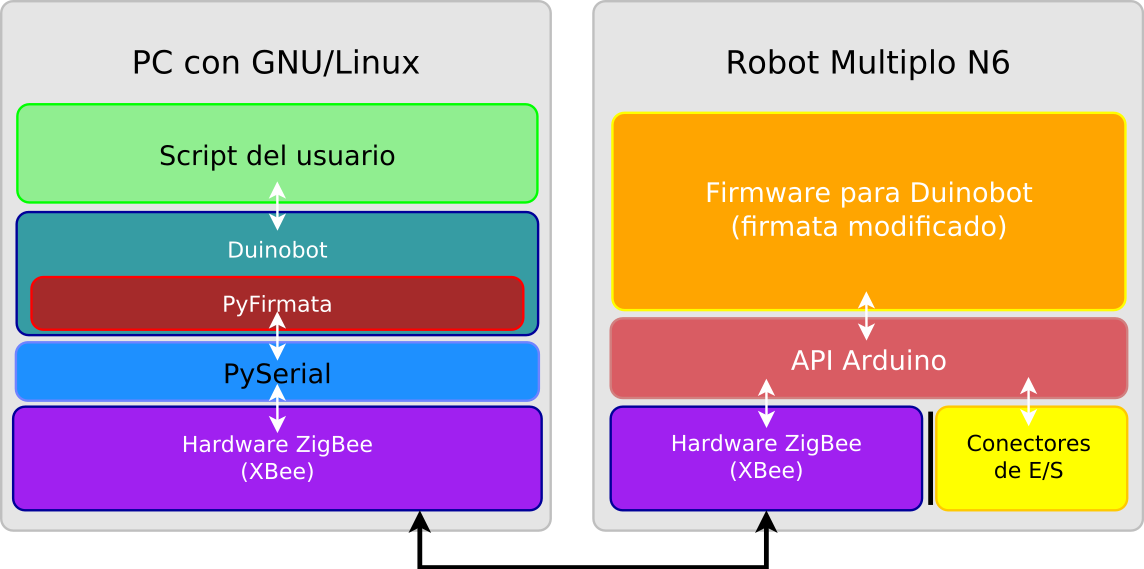
\includegraphics[width=.95\textwidth]{figures/diagrama_duinobot}
        \subcaption{Diagrama de bloques de DuinoBot}
        \label{fig:funcionamiento_duinobot_diagrama}
    \end{subfigure}
    \begin{subfigure}[b]{0.29\textwidth}
        \includegraphics[width=\textwidth]{figures/arquitectura_actual}
        \subcaption{Esquema de conexión típico}
        \label{fig:funcionamiento_duinobot_conexion}
    \end{subfigure}
    \caption{Funcionamiento de DuinoBot}
    \label{fig:funcionamiento_duinobot}
\end{figure}

La modalidad de uso esperada con DuinoBot consiste en que cada usuario
debe contar con una computadora, conectada por USB a una placa XBee,
y desde esa computadora puede controlar uno o más robots. Con esa modalidad
fueron utilizados los robots en los cursos del proyecto
``Programando con robots y software libre'' y en actividades similares
planteadas posteriormente, generalmente además cada alumno controla
un único robot, el esquema de conexión típico en estos cursos se encuentra
ilustrado en la figura~\ref{fig:funcionamiento_duinobot_conexion}.

Como material para los cursos dictados como parte del proyecto \proyecto{}
se escribió un libro de programación con robots que describe por completo
la API de DuinoBot, además de un conjunto de prácticas y diapositivas que pueden
ser reutilizados para dictar cursos similares ya que ese encuentran publicados
con una licencia Creative Commons y disponibles en el sitio del
proyecto\footnote{\url{http://robots.linti.unlp.edu.ar/material_disponible}}.

